%% Copyright 2018 H.\ Rabus
%
% This work may be distributed and/or modified under the
% conditions of the LaTeX Project Public License, either version 1.3
% of this license or (at your option) any later version.
% The latest version of this license is in
%   http://www.latex-project.org/lppl.txt
% and version 1.3 or later is part of all distributions of LaTeX
% version 2005/12/01 or later.
%
% This work has the LPPL maintenance status `author-maintained'.
%
% This work consists of the file texbsp.tex
%

\documentclass[smallheadings]{scrartcl}

%%% GENERAL PACKAGES %%%%%%%%%%%%%%%%%%%%%%%%%%%%%%%%%%%%%%%%%%%%%%%%%%%%%%%%%%
% inputenc allows the usage of non-ascii characters in the LaTeX source code
\usepackage[utf8]{inputenc}
\usepackage{graphicx} 
\usepackage{float}
%\graphicspath{ {/u/hnatiuka/Praktikum/PPI/} }



% title of the document
\title{Bericht zu Serie 5}
% optional subtitle
%\subtitle{Draft from~\today}
% information about the author
\author{%
  Arsen Hnatiuk,\\%
  Max Huneshagen 
}
\date{\today} 


%%% LANGUAGE %%%%%%%%%%%%%%%%%%%%%%%%%%%%%%%%%%%%%%%%%%%%%%%%%%%%%%%%%%%%%%%%%%
% babel provides hyphenation patterns and translations of keywords like 'table
% of contents'
\usepackage[ngerman]{babel}

%%% HYPERLINKS %%%%%%%%%%%%%%%%%%%%%%%%%%%%%%%%%%%%%%%%%%%%%%%%%%%%%%%%%%%%%%%%
% automatic generation of hyperlinks for references and URIs
\usepackage{hyperref}

%%% MATH %%%%%%%%%%%%%%%%%%%%%%%%%%%%%%%%%%%%%%%%%%%%%%%%%%%%%%%%%%%%%%%%%%%%%%
% amsmath provides commands for type-setting mathematical formulas
\usepackage{amsmath}
\numberwithin{equation}{section}
% amssymb provides additional symbols
\usepackage{amssymb}
% HINT
% Use http://detexify.kirelabs.org/classify.html to find unknown symbols!

%%% COLORS %%%%%%%%%%%%%%%%%%%%%%%%%%%%%%%%%%%%%%%%%%%%%%%%%%%%%%%%%%%%%%%%%%%%
% define own colors and use colored text
\usepackage[pdftex,svgnames,hyperref]{xcolor}

%%% Code Listings %%%%%%%%%%%%%%%%
% provides commands for including code (python, latex, ...)
\usepackage{listings}
\definecolor{keywords}{RGB}{255,0,90}
\definecolor{comments}{RGB}{0,0,113}
\definecolor{red}{RGB}{160,0,0}
\definecolor{green}{RGB}{0,150,0}
\lstset{language=Python, 
        basicstyle=\ttfamily\small, 
        keywordstyle=\color{keywords},
        commentstyle=\color{comments},
        stringstyle=\color{red},
        showstringspaces=false,
        identifierstyle=\color{green},
        }


\usepackage{paralist}
\usepackage{nicefrac}
% setting the font style for input und returns in description items
\newcommand{\initem}[2]{\item[\hspace{0.5em} {\normalfont\ttfamily{#1}} {\normalfont\itshape{(#2)}}]}
\newcommand{\outitem}[1]{\item[\hspace{0.5em} \normalfont\itshape{(#1)}]}
\newcommand{\bfpara}[1]{
	
	\noindent \textbf{#1:}\,}


\begin{document}

% generating the title page
\maketitle
% generating the table of contents (requires to run pdflatex twice!)
\tableofcontents
\bigskip

\hrule
\hrule

%%% BEGIN OF CONTENT %%%%%%%%%%%%%%%%%%%%%%%%%%%%%%%%%%%%%%%%%%%%%%%%%%%%%%%%%%

\section{Einleitung}

In dieser Serie soll das bereits in Serie~3 behandelte Problem 
\begin{align}
A^{(d)}\hat{u} = b
\label{eq:glc}
\end{align}
mit $A^{(d)}\in\mathbb{R}^{(n-1)^d\times(n-1)^d}$, $\hat{u},b\in\mathbb{R}^{n-1}$ und der Diskretisierung $n\in\mathbb{N}$ sowie $\hat{u},b \in \mathbb{R}^{(n-1)^d}$ erneut aufgegriffen werden. Dieses ist durch eine bestimmte Wahl von $A^{(d)}$ und $b$, die in Serie~2 erläutert wurde,  eine diskrete Formulierung des Laplace-Problems 
\begin{align}
\begin{split}
-\Delta u&=f(x)\text{ in }\Omega=(0, 1)^d, d\in\{1,2,3\}\\
u \vert _{\partial\Omega}&=u_D\text{ für ein gegebenes }u_D.
\end{split}
\label{eq:rwp}
\end{align}
Das exakte Lösen von \eqref{eq:glc} kann für feine Diskretisierungen einen sehr hohen Rechenaufwand verursachen. Im Laufe dessen wurde in Serie~3 die  $L$-$U$-Zerlegung von $A^{(d)}$ berechnet. Während $A^{(d)}$ eine Banddiagonalmatrix ist und sich demzufolge gut als \textit{sparse}-Matrix speichern lässt, ist dies für $L$ und $U$ im Allgemeinen nicht der Fall. Dieser Speicherplatzvorteil kann also bei der Verwendung der $L$-$U$-Zerlegung nicht länger ausgenutzt werden. Diese Beobachtungen motivieren die Verwendung von iterativen Verfahren wie der \emph{conjugate gradients}-Methode (\textbf{CG}). Bei dieser handelt es sich eigentlich um ein exaktes Verfahren, mit dem sich ein Gleichungssystem der Form
\begin{align}
Bx=d
\end{align}
mit $B \in \mathbb{R}^{m\times m}$ s.\,p.\,d. und $x,d\in \mathbb{R}^m$ in $m$ Iterationsschritten exakt lösen lässt. In der Praxis kann das Verfahren aber meist nach viel weniger Schritten abgebrochen werden, da die Zwischenlösung schon nahe genug (insbesondere im Vergleich zum Diskretisierungsfehler) an der exakten Lösung liegt.

Die \textbf{CG}-Methode soll im Folgenden verwendet werden, um \eqref{eq:rwp} für ein vorgegebenes $u$ bzw. \eqref{eq:glc} für eine vorgegebene rechte Seite näherungsweise zu lösen. Die so erhaltene approximative Lösung wird mit der Lösung mit dem bereits in Serie~3 verwendeten Verfahren hinsichtlich des Konvergenzverhaltens verglichen. 

\section{Theorie}


Sei $B \in \mathbb{R}^{m\times m}$ s.\,p.\,d. und $x,d\in \mathbb{R}^m$. Sei $x_0\in \mathbb{R}^m$ beliebig. Dann berechnet sich eine Lösung von $Bx=d$ wie folgt \cite{wiki:cg}:

%TODO Hier eventuell Einzug?

Zunächst sei 
\begin{align}
r_0&:=d-Bx_0\\
d_0&:=r_0.
\end{align}
Berechne nun für $k=0,1,2,\dots$:
\begin{align}
z&=Bd_k,\\
\alpha&=\frac{r_k^Tr_k}{d_k^Tz},\\
x_{k+1}&=x_k+\alpha_kd_k,\\
r_{k+1}&=r_k-\alpha_kz,\\
\beta_k&=\frac{r^T_{k+1}r_{k+1}}{r^T_{k}r_{k}},\\
d_{k+1}&=r_{k+1}+\beta_kd_k,
\end{align}
bis das Residuum $\|r_{k+1}\|_\infty$ kleiner als ein zuvor gegebenes $\epsilon$ wird.
Zu prüfen ist nun noch, ob die Matrizen $A^{(d)}$ die o.\,g. Bedingungen erfüllen und symmetrisch und positiv semidefinit sind. Symmetrie folgt direkt aus der Definition der Matrizen, die positive Definitheit folgt daraus, dass die $A^{(d)}$ streng diagonaldominante Matrizen sind, also dass gilt:
\begin{align}
|(A^{(d)})_{ii}|> \sum\limits_{\substack{j=1 \\j\neq i}}|(A^{(d)})_{ij}|.
\end{align}
Dies ist gegeben, da die Diagonaleinträge von $A^{(d)}$ den Betrag $2d$ (s.~Serie~2) haben und sich in jeder Zeile höchstens $d$ Einträge mit dem Betrag $1$ befinden, während die restlichen Beiträge $0$ sind. Benutzt man nun noch, dass alle Diagonaleinträge von $A^{(d)}$ stets positiv sind, so folgt daraus, dass diese Metrizen positiv definit sind \cite{skript:nla}. Demzufolge lässt sich die CG-Methode auf diese Matrizen anwenden. 



\section{Experimente}

Es wurden Experimente durchgeführt, um das Konvergenzvehalten der \textit{C-G-Methode} zu bestimmen.

%\begin{figure}[H]
%	\centering
%	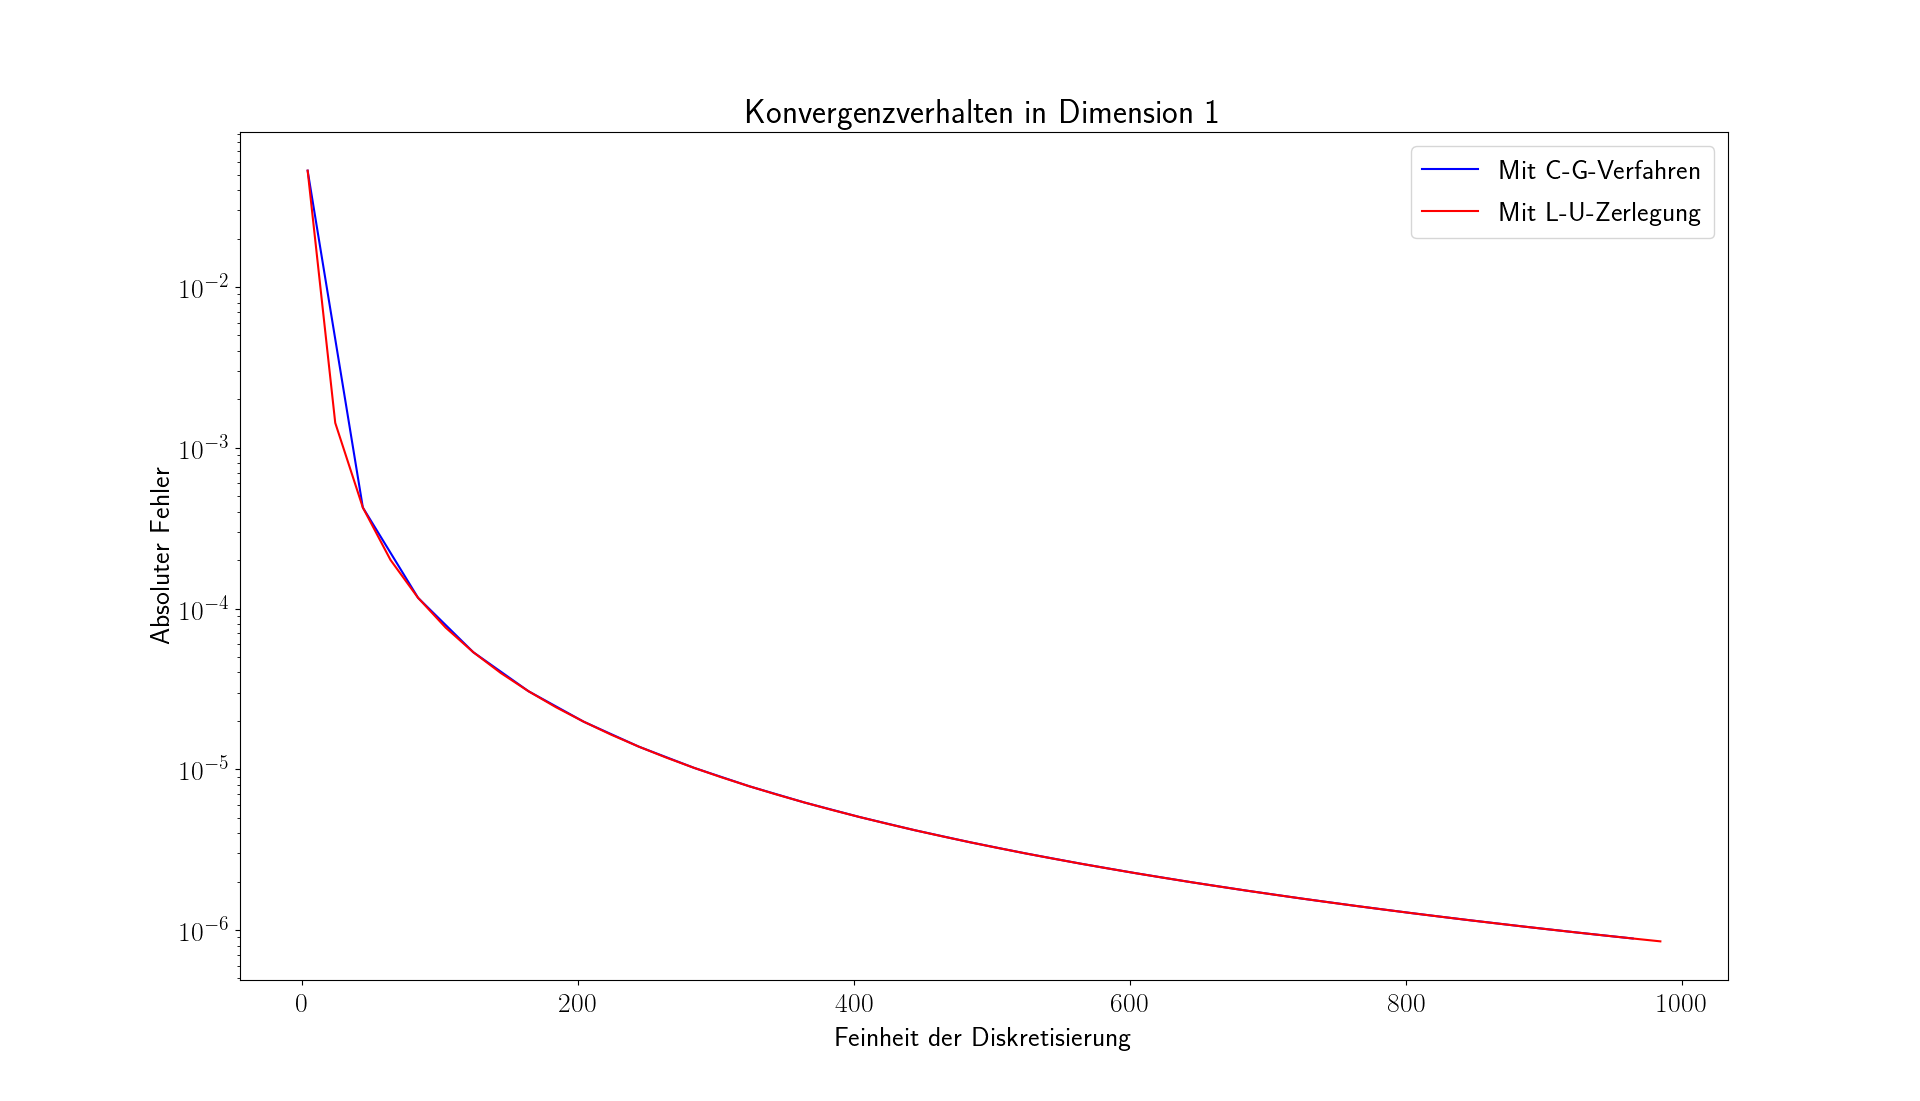
\includegraphics[width=\linewidth]{Bilder/VergleichDim1}
%	\caption{Vergleich der Genauigkeit der zwei implementierten Methoden in der ersten Dimension}
%	\label{fig:vergleichdim1}
%\end{figure}
%
%\begin{figure}[H]
%	\centering
%	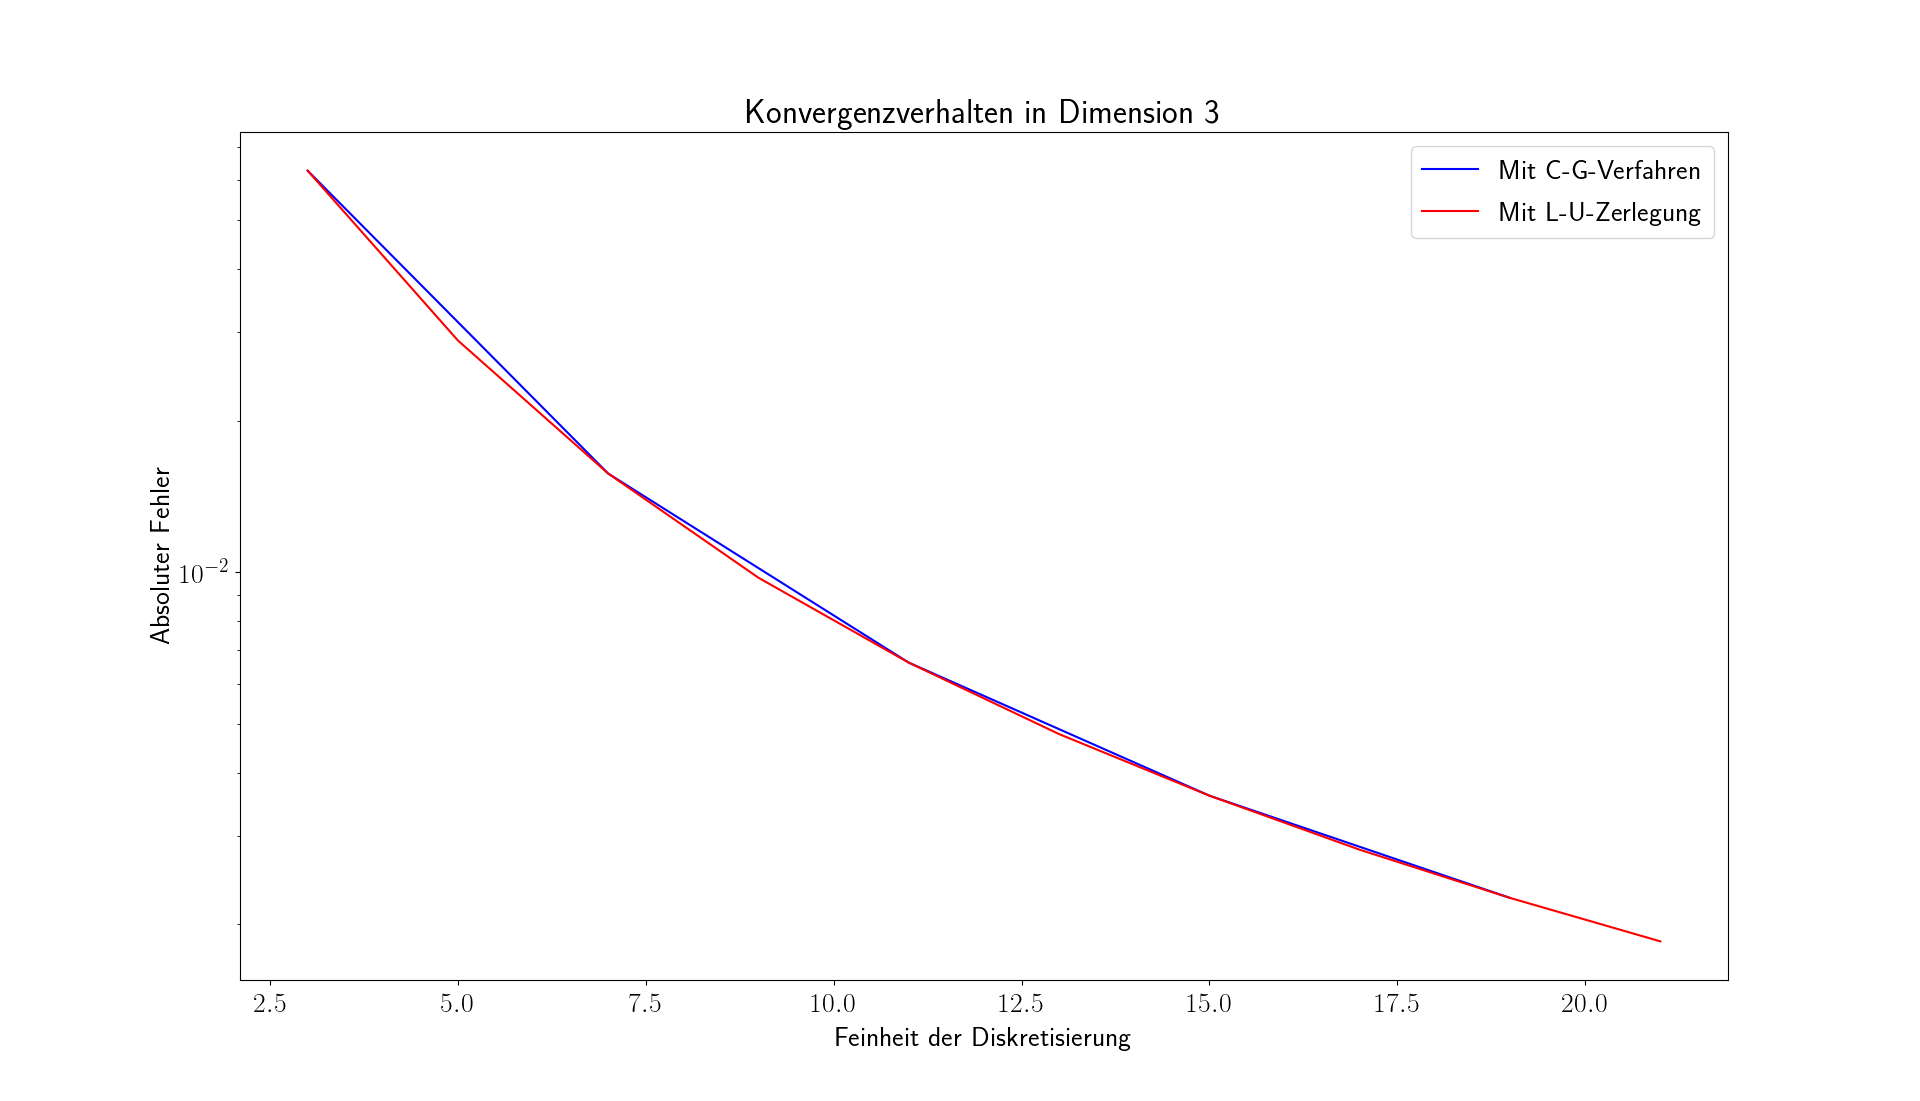
\includegraphics[width=\linewidth]{Bilder/VergleichDim3}
%	\caption{Vergleich der Genauigkeit der zwei implementierten Methoden in der dritten Dimension}
%	\label{fig:vegleichdim3}
%\end{figure}

\begin{figure}[H]
\centering
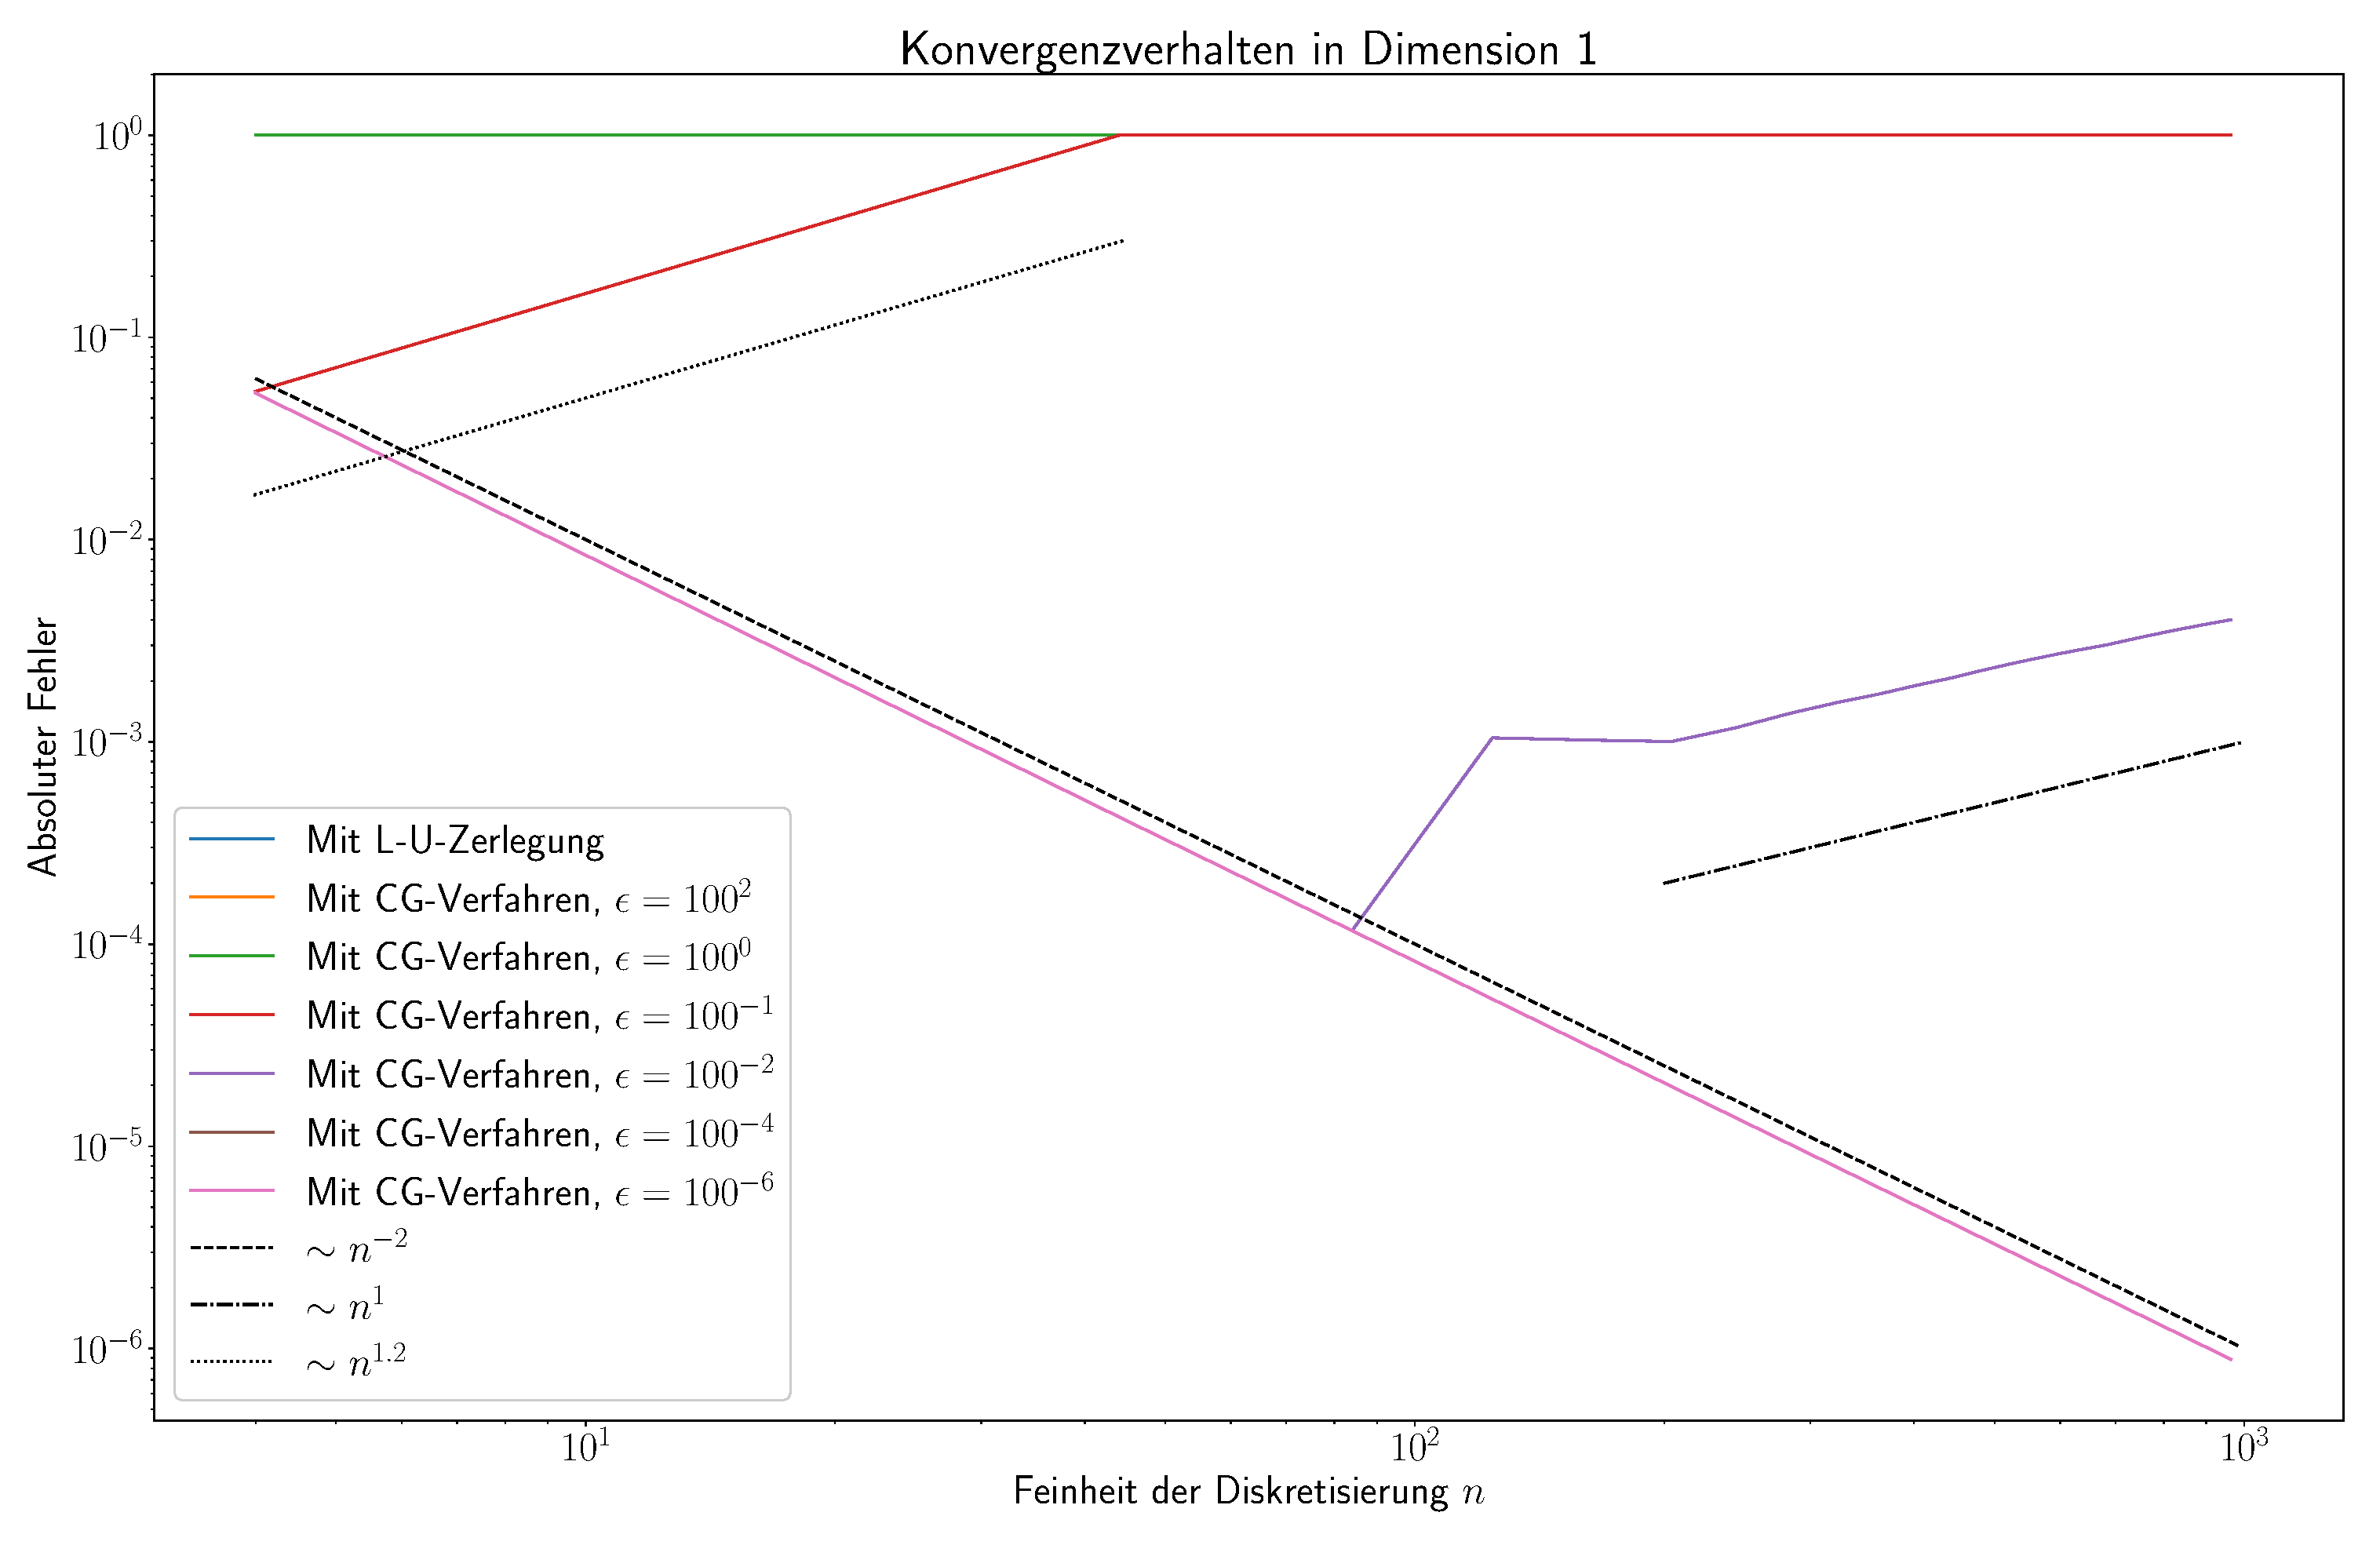
\includegraphics[width=\textwidth]{Bilder/KonVerh_dim_1.eps}
\caption{Vergleich der Genauigkeit der zwei implementierten Methoden für eine Dimension}
\label{fig:vergleichdim1}
\end{figure}

In Abb.~\ref{fig:vergleichdim1} wurde das Konvergenzverhalten in einer Dimension für verschiedene $\epsilon$ in Abhängigkeit von der Feinheit der Diskretisierung $n=\nicefrac{1}{h}$ geplottet. Wie erwartet sinkt der absolute Fehler nicht unter $\epsilon$. Stattdessen kommt es zu \glqq Abzweigungen\grqq, wenn der absolute Fehler sich $\epsilon$ annähert. Für $\epsilon\leq 100^{-4}=10^{-8}$  ist das Konvergenzverhalten im untersuchten Bereich für alle $\epsilon$ gleich und deckt sich mit dem Verhalten der Lösung, die mittels der L-U-Zerlegung ermittelt wurde. Dieser gemeinsame Verlauf ist in der doppeltlogarithmischen Darstellung von Abb.~\ref{fig:vergleichdim1} parallel zu $n^{-2}$, die Abzweigung für $\epsilon=10^{-4}$ ist für $10^{2.3} \leq n\leq 10^{3}$ in etwa parallel zu  $n^{1}$, während die $\epsilon=10^{-2}$-Abzweigung sich wie $n^{1.2}$ verhält, bis sie etwa ab $n=10^{1.65}$ konstant bei 1 verharrt. Es kann also bei hinreichend großen Fehlerschranken passieren, dass das Problem für feiner werdende Diskretisierungen schlechter gelöst wird, ansonsten sinkt der absolute Fehler mit steigendem $n$. Für sehr große $\epsilon \geq 1$ liegt der Fehler konstant bei 1, da schon bei der der nullten Iteration abgebrochen wird, der Startwert liegt also schon nahe genug an der tatsächlichen Lösung. 

%Die Figuren \ref{fig:vergleichdim1} und \ref{fig:vegleichdim3} waren mit der festen Abbruchsschranke $10^{-14 }$ erzeugt und zeigen, dass das  \textit{CG-Verfahren} nach ausreichend viele Iterationen auf ein Ergebnis kommt, das nur durch den Fehler der Diskretisierung geprägt wird. Dies siehr man noch besser in \ref{fig:iterdim1} und \ref{fig:iterdim3}.

\begin{figure}[H]
	\centering
	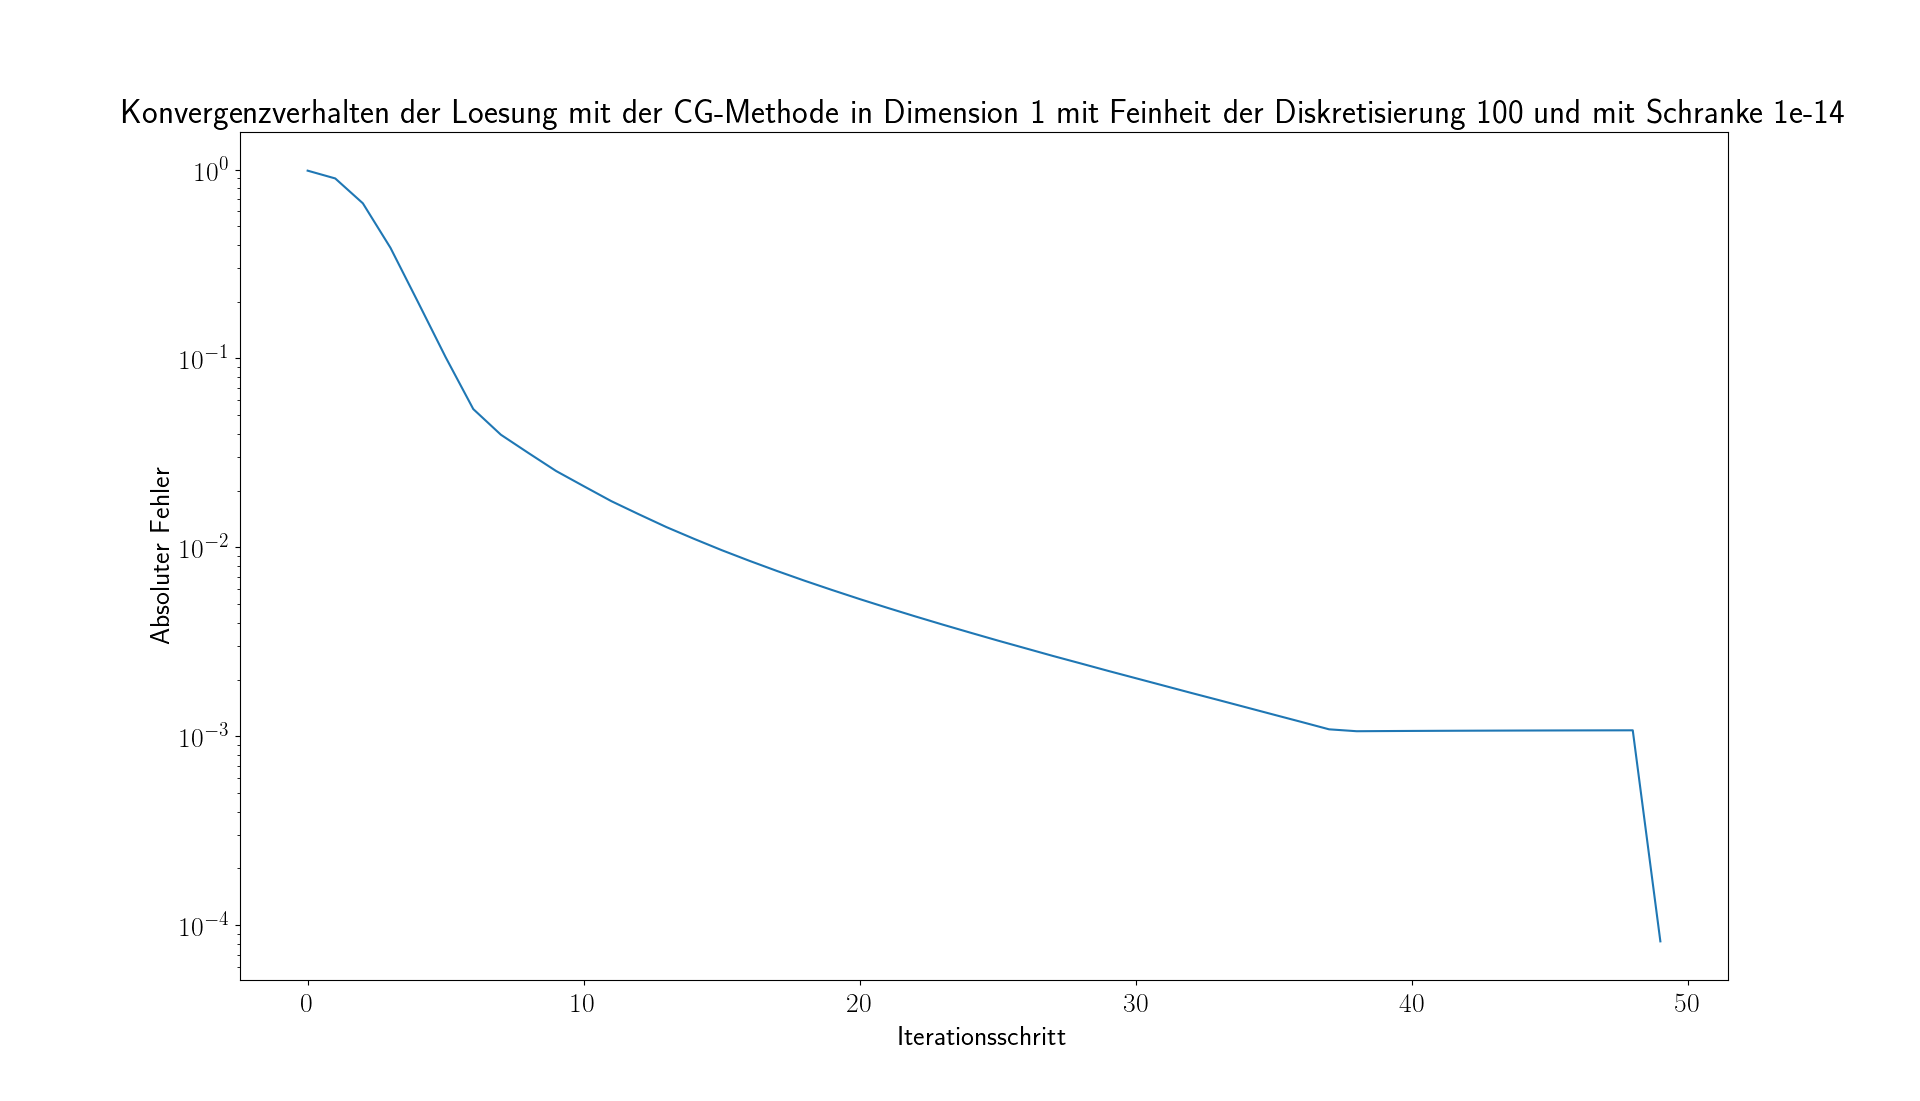
\includegraphics[width=\linewidth]{Bilder/IterDim1}
	\caption{Der Fehler bezüglich des Iterationsschritts im CG-Verfahren für eine Dimension}
	\label{fig:iterdim1}
\end{figure}

\begin{figure}[H]
	\centering
	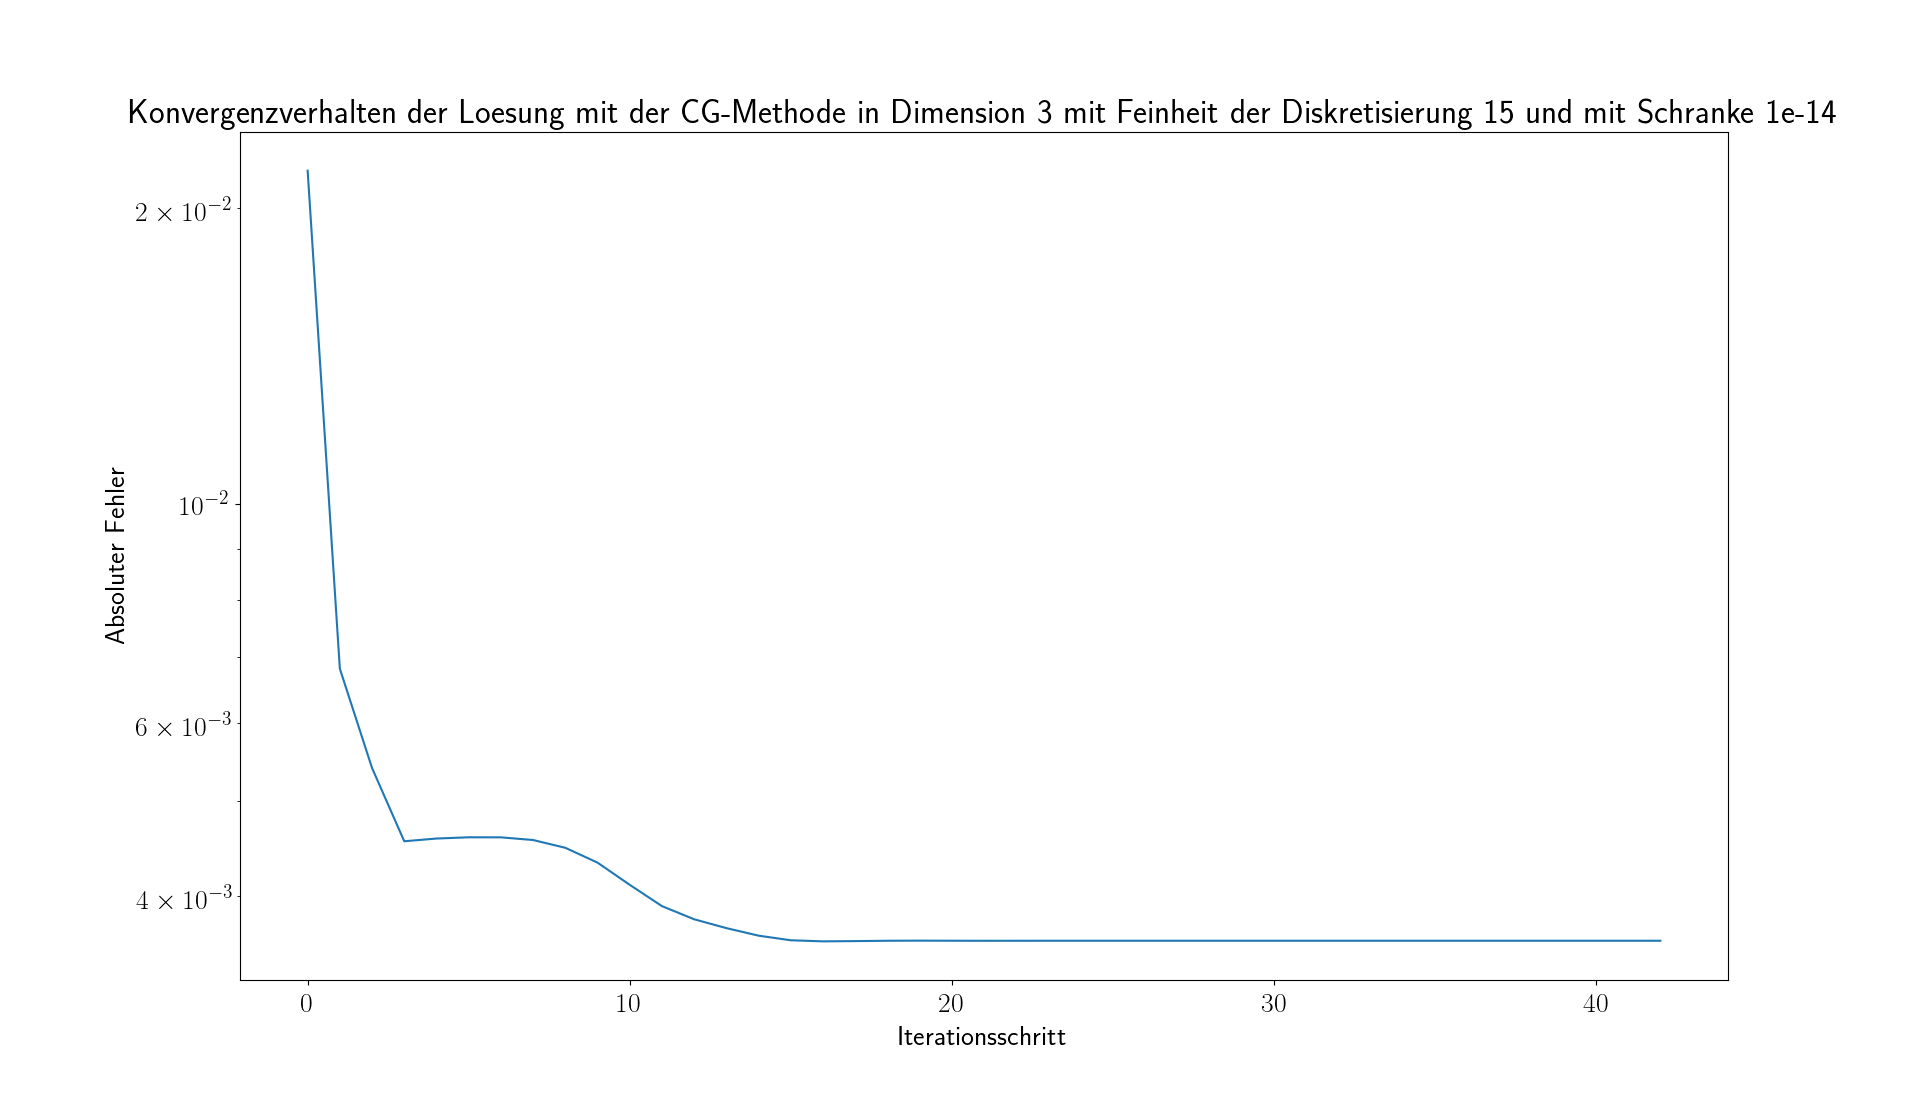
\includegraphics[width=\linewidth]{Bilder/IterDim3}
	\caption{Der Fehler bezüglich des Iterationsschritts im CG-Verfahren in drei Dimensionen}
	\label{fig:iterdim3}
\end{figure}
 
Die Abb.~\ref{fig:iterdim1}  und~\ref{fig:iterdim3} zeigen, dass der Fehler in der durch die \textit{CG-Methode} nach genügend vielen Iterationen gewonnene Lösung durch den Fehler der Diskretisierung dominiert wird. Obwohl in beiden Fällen das Residuum in der Iteration am Ende kleiner als $10^{-14}$ ist, bleibt der absolute Fehler in \ref{fig:iterdim1} bei $10^{-4}$ und in \ref{fig:iterdim3} bei $10^{-3}$. Genau diese Werte sind die Fehler der Diskretisierung für Dimension 1 und Feinheit 100 bzw. Dimension 3 und Feinheit 15 (vgl. auch  \ref{fig:vergleichdim1}). Eine weitere Beobachtung von den Abbildungen \ref{fig:iterdim1} und \ref{fig:iterdim3} ist dass die Konvergenz der \textit{CG-Methode} immer mit einem Sprung endet. Aus der Theorie wissen wir, dass der exakte Wert nach höchstens $dim(Matrix)$-vielen Iterationsschritten gewonnen ist, und das ist auch bei unseren Ergebnissen der Fall. Die Konvergenz erfolgt in der Tat nach deutlich weniger als $dim(Matrix)$-vielen Schritten (ungefähr 50 anstelle von 100 in einer Dimension und 15 anstelle von $15^3=3375$) .Jedoch sehen wir auch, dass sofern ein Zwischenergebnis in einer geeigneter Umgebung der exakten Ergebnis liegt, konvergiert das Verfahren fast instantan.  Dies ist insbesondere in \ref{fig:iterdim1} sichtbar. Bei einer Wahl von dem Nullvektor als Startwert in der Iteration konvergiert das Verfahren sogar in ein Schritt. Deswegen wird hier der Vektor mit Werten $0.001$ als Startwert verwendet. 
 
 \begin{figure}[H]
 	\centering
 	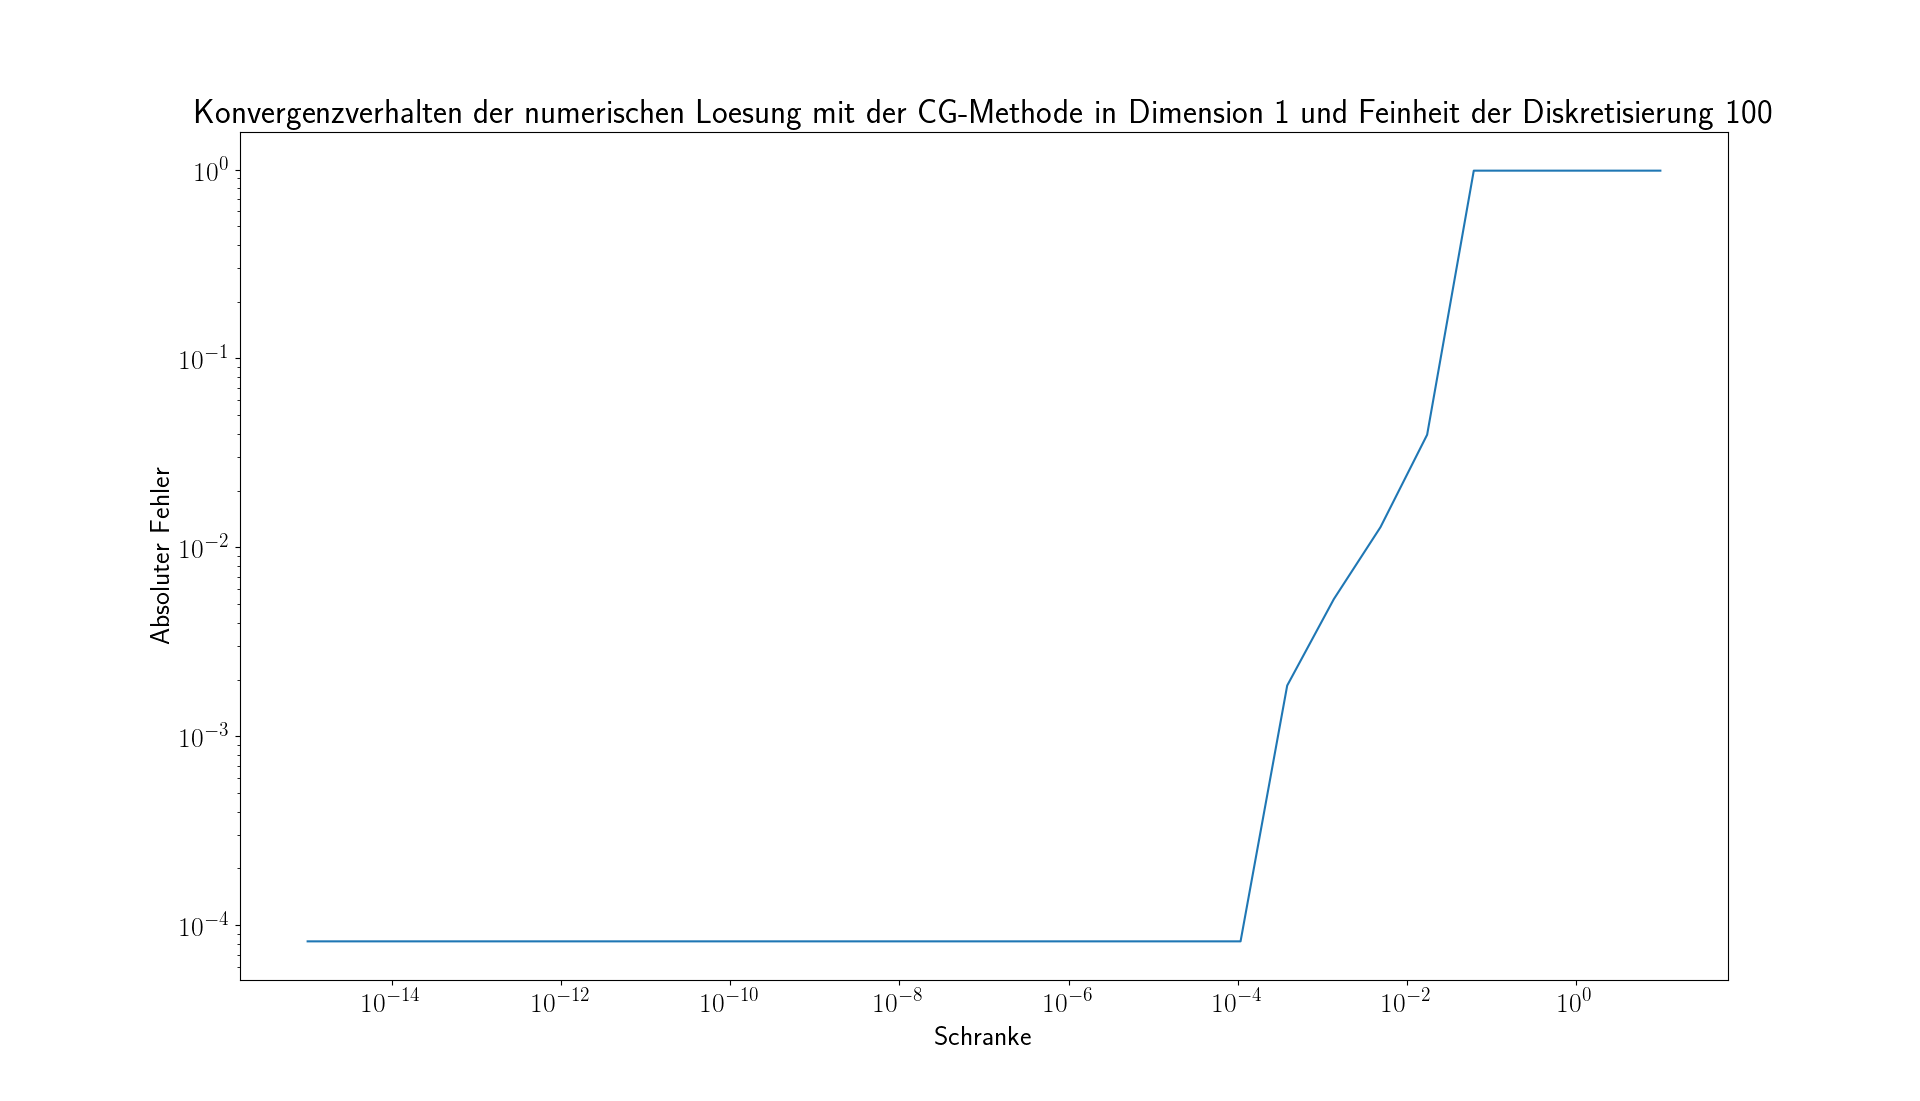
\includegraphics[width=\linewidth]{Bilder/SchranekDim1}
 	\caption{Der Fehler bezüglich der Abbruchsschranke im CG-Verfahren in einer Dimension}
 	\label{fig:schrankedim1}
 \end{figure}

 \begin{figure}[H]
 	\centering
 	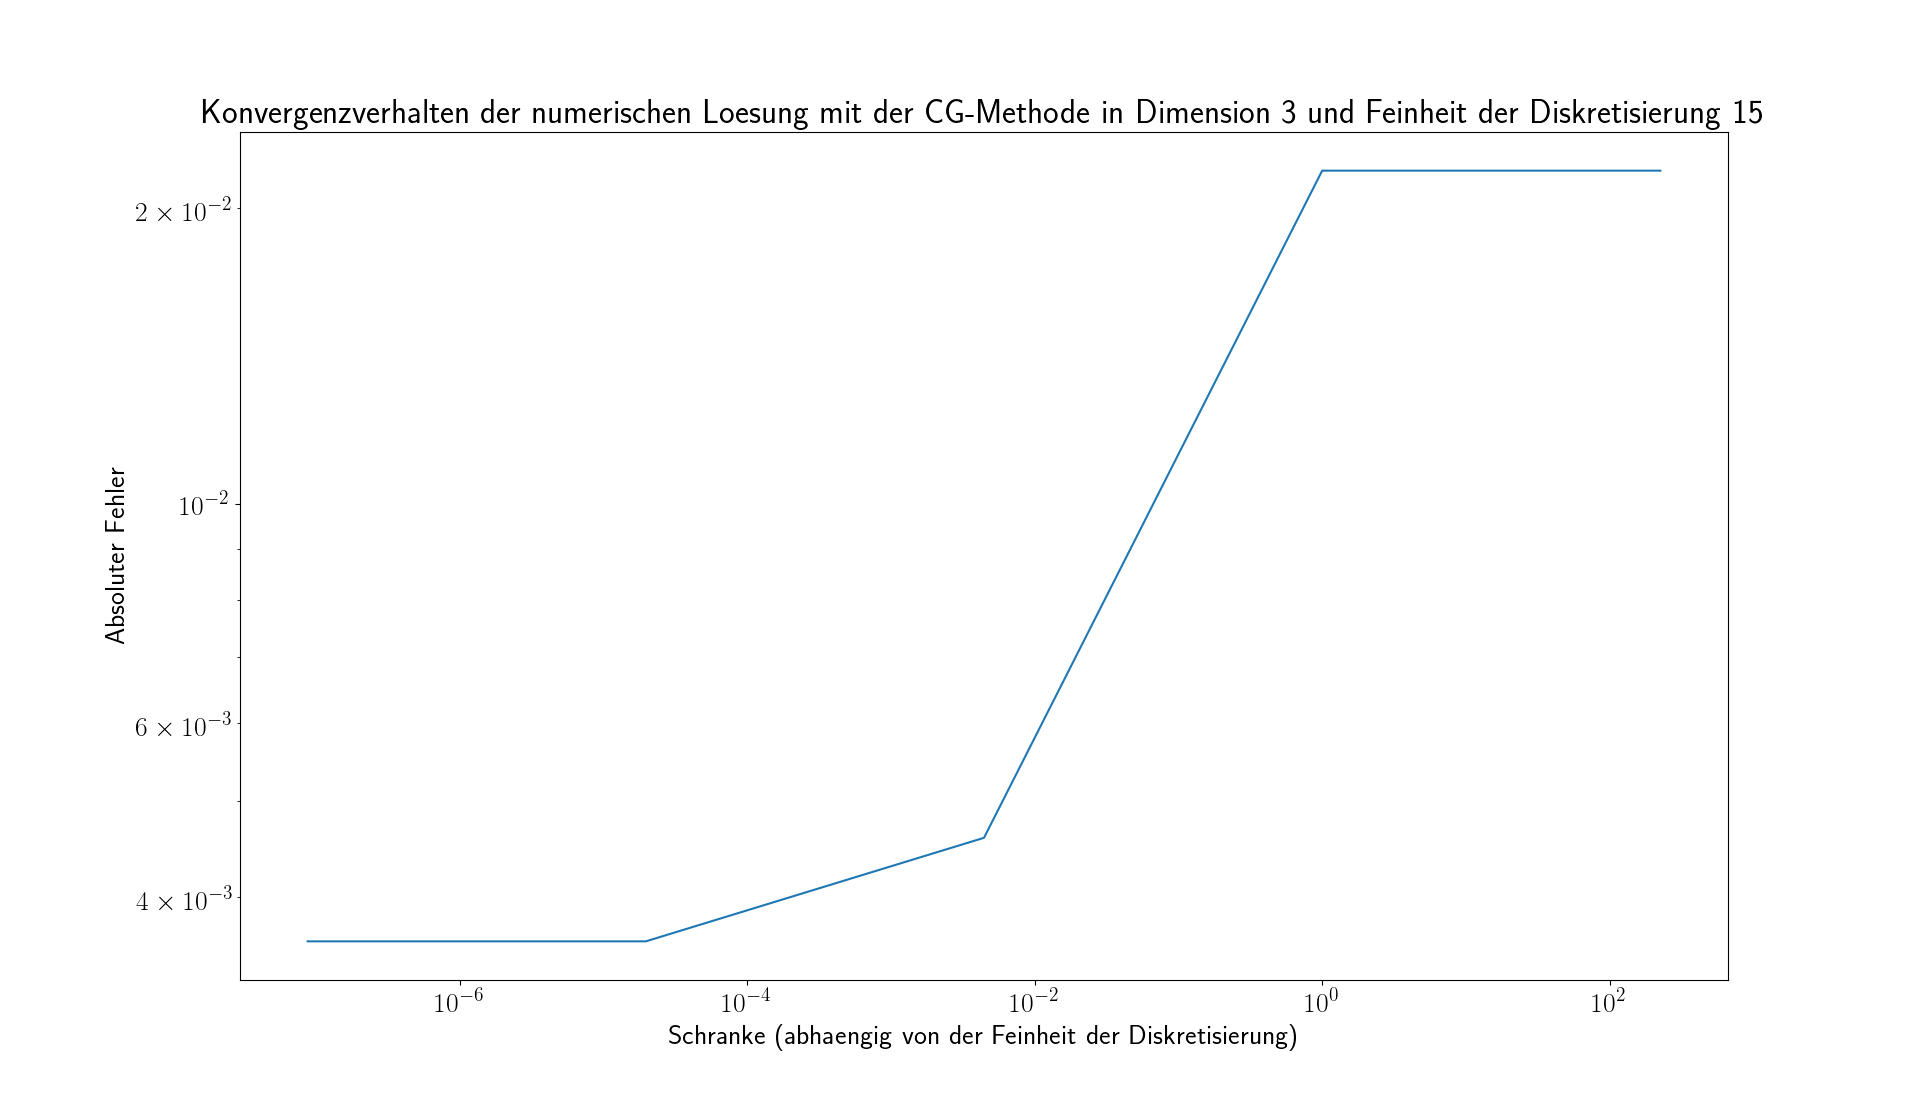
\includegraphics[width=\linewidth]{Bilder/loglogdim3}
 	\caption{Der Fehler bezüglich der Abbruchsschranke als Funktion der Feinheit der Diskretisierung im CG-Verfahren in drei Dimensionen}
 	\label{fig:loglog3}
 \end{figure}

Die Abbildungen \ref{fig:schrankedim1} und \ref{fig:loglog3} zeigen erneut, dass der Fehler im \textit{CG-Verfahren} durch den Fehler der Diskretisierung von unten beschränkt ist. Ab einer bestimmten Wahl von der Abbruchsschranke wird das Ergebnis nicht mehr verbessert, weil die Genauigkeit stärker von der Diskretisuerung geprägt wird. In Figur \ref{fig:loglog3} ist die Schranke als $n^{-k}$ gesetzt, wobei $n$ die Feinheit der Diskretisierung ist und $k$ eine Natürliche Zahl zwischen -2 und 6 ist. Wie erwartet, spielt die Wahl der Schranke ab einem bestimmten Punkt (um $10^{-3}$)keine Rolle mehr.

\section{Zusammenfassung}

Das \textit{CG-Verfahren} hat sich als eine zuverlässige Lösungsmethode des Laplace-Problems herausgestellt. Die exakte Lösung wird nach verhältnismäßig wenig Iterationsschritten gewonnen. Jedoch ist es wichtig, eine nicht zu große Abbruchsschranke anzugeben, weil viele Iterationen könnten dann Sinnlos sein, da die Genauigkeit des Ergebnis sowieso durch den Diskretidierungsfehler beschränkt ist.

\begin{thebibliography}{9}
\bibitem{wiki:cg} Kein Autor, Aufgerufen am \today, \textit{CG-Verfahren}. 
\url{https://de.wikipedia.org/wiki/CG-Verfahren}
\bibitem{skript:nla} Axel~Kröner: Vorlesungsskript \textit{Numerische Lineare Algebra}, WS 2018/19. 
\url{https://moodle.hu-berlin.de/pluginfile.php/2445740/mod_resource/content/25/Skriptum_NLA.pdf} (passwortgeschützt)
\end{thebibliography}


%%% END OF DOCUMENT %%%%%%%%%%%%%%%%%%%%%%%%%%%%%%%%%%%%%%%%%%%%%%%%%%%%%%%%%%%
\end{document}
